\subsection{Вкладка: Монитор}

Окно монитора отображает данные о произошедших событиях в табличном виде.
Чтобы просмотреть только информацию о метках, необходимо поставить флажок <<только информация о метках>>.
По нажатию на кнопку <<Очистить>>, происходит удаление всех записей в таблице монитора.
По нажатию на кнопку <<Сохранить>>, вызывается диалог с выбором имени файла для сохранения таблицы монитора в
csv файл, который легко открывается программой Microsoft Office Excel.

\begin{center}
    
\includegraphics[scale=0.5]{img/monitor.png}
\end{center}

\subsection{Вкладка: Параметры фильтрации}

На данной вкладке задаются параметры поиска событий в таблице монитора. 
При переключении на вкладку монитора, выполняется мгновенный поиск в соответствии с заданными параметрами.
Результаты отображаются в таблице монитора, которые можно сохранить в виде отчета в файл csv, а затем открыть и распечатать,
при необходимости, в Microsoft Office Excel.

\begin{center}
    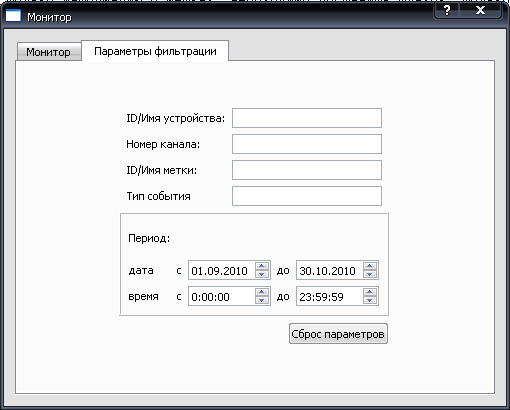
\includegraphics[scale=0.5]{img/monitor_find.png}
\end{center}